\documentclass[final]{beamer}
%% Possible paper sizes: a0, a0b, a1, a2, a3, a4.
%% Possible orientations: portrait, landscape
%% Font sizes can be changed using the scale option.
\usepackage[size=a0,orientation=portrait,scale=1.3]{beamerposter}

\usetheme{gemini}
\usecolortheme{seagull}
\useinnertheme{rectangles}

% ====================
% Packages
% ====================

\usepackage[utf8]{inputenc}
\usepackage{graphicx}
\usepackage{bm, amsmath}
\usepackage{hyperref}
\graphicspath{{./../../DALE/ACML-poster}}
\hypersetup{
    colorlinks=true,
    linkcolor=blue,
    filecolor=magenta,      
    urlcolor=cyan,
    pdftitle={Overleaf Example},
    pdfpagemode=FullScreen,
    }
% \usepackage[most]{tcolorox}
\usepackage{wrapfig}
\usepackage{booktabs}
\usepackage{tikz}
\usepackage{pgfplots}

\newcommand{\xb}{\mathbf{x}}

% ====================
% Lengths
% ====================

% If you have N columns, choose \sepwidth and \colwidth such that
% (N+1)*\sepwidth + N*\colwidth = \paperwidth
\newlength{\sepwidth}
\newlength{\colwidth}
\setlength{\sepwidth}{0.03\paperwidth}
\setlength{\colwidth}{0.45\paperwidth}

\newcommand{\separatorcolumn}{\begin{column}{\sepwidth}\end{column}}

% ====================
% Logo (optional)
% ====================

% LaTeX logo taken from https://commons.wikimedia.org/wiki/File:LaTeX_logo.svg
% use this to include logos on the left and/or right side of the header:
\logoright{
\includegraphics[height=5cm]{logos/athena-278x300.png}}
\logoleft{
\includegraphics[height=4cm]{logos/dit-logo.png}}

% ====================
% Footer (optional)
% ====================

\footercontent{
	ECAI 2023, Krakow, Poland \hfill
	\insertdate \hfill
	\href{mailto:vgkolemis@athenarc.gr}{\texttt{vgkolemis@athenarc.gr}}
}
% (can be left out to remove footer)

% ====================
% My own customization
% - BibLaTeX
% - Boxes with tcolorbox
% - User-defined commands
% ====================
% ====================
% BibLaTeX
% ====================

\usepackage[backend=biber,
	bibstyle=authoryear,
	citestyle=authoryear,
	style=authoryear,
	maxcitenames=2,
	maxbibnames=20, % limit the length of list of names (authors/editors/etc.)
	sorting=ydnt, % sort references by year (descending), name, title
	dashed=false, % show authors instead of dash in publications having the same authors
	giveninits=true % render authors' given name initials and not the full given names
]{biblatex}
%% Biblatex with Beamer bibliography icons
\setbeamertemplate{bibliography item}{%
	\ifboolexpr{ test {\ifentrytype{book}} or test {\ifentrytype{mvbook}}
		or test {\ifentrytype{collection}} or test {\ifentrytype{mvcollection}}
		or test {\ifentrytype{reference}} or test {\ifentrytype{mvreference}} }
	{\setbeamertemplate{bibliography item}[book]}
	{\ifentrytype{online}
		{\setbeamertemplate{bibliography item}[online]}
		{\setbeamertemplate{bibliography item}[article]}}%
	\usebeamertemplate{bibliography item}}
\defbibenvironment{bibliography}
{\list{}
	{\settowidth{\labelwidth}{\usebeamertemplate{bibliography item}}%
		\setlength{\leftmargin}{\labelwidth}%
		\setlength{\labelsep}{\biblabelsep}%
		\addtolength{\leftmargin}{\labelsep}%
		\setlength{\itemsep}{\bibitemsep}%
		\setlength{\parsep}{\bibparsep}}}
{\endlist}
{\item}
%% Redefine \refname
\renewcommand{\bibname}{References}
%% Redefine \parencite to use square brackets instead of braces
\DeclareCiteCommand{\parencite}
{\usebibmacro{prenote}}
{\usebibmacro{citeindex}%
	\printtext[bibhyperref]{[\usebibmacro{cite}]}}
{\multicitedelim}
{\usebibmacro{postnote}}
%% Highlight author names using Beamer data annotation
%% Usage: add a new line `author+an = {<author-order>=highlight}` to an entry
%% For example: author+an = {3=highlight} => highlight the 3rd author name
\AtBeginBibliography{
	\renewcommand*{\mkbibnamegiven}[1]{%
		\ifitemannotation{highlight}
		{\textbf{#1}}
		{#1}%
	}
	
	\renewcommand*{\mkbibnamefamily}[1]{%
		\ifitemannotation{highlight}
		{\textbf{#1}}
		{#1}%
	}
}

% ====================
% Boxes with tcolorbox
% ====================
\usepackage[most]{tcolorbox}

%%% Beamer colors in boxes

\newcommand{\beamercolorsinboxes}[1]{
	\setbeamercolor{itemize item}{fg=#1!75!black}
	\setbeamercolor{itemize/enumerate body}{fg=#1!65!white}
	\setbeamercolor{itemize/enumerate subbody}{fg=#1!65!white}
	\setbeamercolor{item projected}{fg=white, bg=#1!75!black}
}

%%% Highlight Oval Box
\newtcbox{\xmybox}[1][red]{on line,
	arc=7pt,colback=#1!10!white,colframe=#1!50!black,
	before upper={\rule[-3pt]{0pt}{10pt}},boxrule=1pt,
	boxsep=0pt,left=6pt,right=6pt,top=2pt,bottom=2pt}
%%% Box for stating problems
%%%%%%%%
%Usage: (similar for infobox)
%	\begin{defbox}{title}
	%		contents
	%	\end{defbox}
%%%%%%%%
\newtcolorbox{defbox}[1]{%
	enhanced,
	attach boxed title to top 	left={xshift=5mm,yshift=-5mm,yshifttext=-5mm},
	colback=cyan!5!white,
	colframe=cyan!75!black,
	coltitle=cyan!80!black,
%	left=0mm,right=0mm,top=2mm,bottom=0mm,
	title={#1},
	fonttitle=\bfseries\large, fontupper=\color{cyan!65!white},
	boxed title style={colback=cyan!5!white,colframe=cyan!75!black},
	before upper={
		\beamercolorsinboxes{cyan}
	}
}%
%%% Box for announcement
\newtcolorbox{infobox}[1]{%
	enhanced,
	attach boxed title to top 	left={xshift=5mm,yshift=-5mm,yshifttext=-5mm},
	colback=yellow,
	colframe=red!75!black,
	coltitle=red!75!black,
%	left=0mm,right=0mm,top=2mm,bottom=0mm,
	title={#1},
	fonttitle=\bfseries\large, fontupper=\color{red!65!white},
	boxed title style={colback=yellow,colframe=red!75!black},
	before upper={
		\beamercolorsinboxes{red}
	}
}%
%%% Box for example
\newtcolorbox{exabox}[1]{%
	enhanced,
	attach boxed title to top 	left={xshift=5mm,yshift=-5mm,yshifttext=-5mm},
	colframe=brown!75!black,colback=brown!5!white,coltitle=brown!50!brown!75!black,
%	left=0mm,right=0mm,top=2mm,bottom=0mm,
	title={#1},
	fonttitle=\bfseries\large, fontupper=\color{brown!65!white},
	boxed title style={colback=brown!5!white,coltitle=brown!50!brown!75!black},
	before upper={
		\beamercolorsinboxes{brown}
	}
}%
%%% Theorem Box
%%%%%%%%
%Usage: (similar for conjecture, lemma, etc.)
%	\begin{thm}{title}{nameref}
	%		contents
	%	\end{thm}
% Use \ref{thm:nameref} to refer to the theorem
%%%%%%%%
%%%% Use \newtcbtheorem[number within=section]{thm} to number within each section
\newtcbtheorem[]{thm}%
{Theorem}{attach boxed title to top 	left={xshift=5mm,yshift=-5mm,yshifttext=-5mm},
	enhanced jigsaw,
	%	top=2mm,bottom=0mm,left=0mm,right=0mm,
	fonttitle=\bfseries\large,fontupper=\itshape\color{blue!65!white},
	colframe=blue!75!black,colback=blue!5!white,coltitle=blue!50!blue!75!black,
	boxed title style={colback=blue!5!white,coltitle=blue!50!blue!75!black},
	before upper={
		\beamercolorsinboxes{blue}
	}
}{thm}%
%%% Proposition Box
\newtcbtheorem[use counter from=thm]{prop}%
{Proposition}{attach boxed title to top 	left={xshift=5mm,yshift=-5mm,yshifttext=-5mm},
	enhanced jigsaw,
	%	top=2mm,bottom=0mm,left=0mm,right=0mm,
	fonttitle=\bfseries\large,fontupper=\itshape,
	colframe=gray!75!black,colback=gray!5!white,coltitle=gray!50!gray!75!black,
	boxed title style={colback=gray!5!white,coltitle=gray!50!gray!75!black},
	before upper={
		\beamercolorsinboxes{gray}
	}
}{prop}%
%%% Conjecture Box
\newtcbtheorem[use counter from=thm]{conj}%
{Conjecture}{attach boxed title to top 	left={xshift=5mm,yshift=-5mm,yshifttext=-5mm},
	enhanced jigsaw,
	%	top=2mm,bottom=0mm,left=0mm,right=0mm,
	fonttitle=\bfseries\large,fontupper=\slshape,
	colframe=orange!75!black,colback=orange!5!white,coltitle=orange!50!orange!75!black,
	boxed title style={colback=orange!5!white,coltitle=orange!50!orange!75!black},
	before upper={
		\beamercolorsinboxes{orange}
	}
}{conj}%
%%% Lemma Box
\newtcbtheorem[use counter from=thm]{lem}%
{Lemma}{attach boxed title to top 	left={xshift=5mm,yshift=-5mm,yshifttext=-5mm},
	enhanced jigsaw,
	%	top=2mm,bottom=0mm,left=0mm,right=0mm,
	fonttitle=\bfseries\large,fontupper=\itshape,
	colframe=green!75!black,colback=green!5!white,coltitle=green!50!green!75!black,
	boxed title style={colback=green!5!white,coltitle=green!50!green!75!black},
	before upper={
		\beamercolorsinboxes{green}
	}
}{lem}%
%%% Claim Box
\newtcbtheorem[use counter from=thm]{clm}%
{Claim}{attach boxed title to top 	left={xshift=5mm,yshift=-5mm,yshifttext=-5mm},
	enhanced jigsaw,
	%	top=2mm,bottom=0mm,left=0mm,right=0mm,
	fonttitle=\bfseries\large,fontupper=\itshape,
	colframe=pink!75!black,colback=pink!5!white,coltitle=pink!50!pink!75!black,
	boxed title style={colback=pink!5!white,coltitle=pink!50!pink!75!black},
	before upper={
		\beamercolorsinboxes{pink}
	}
}{clm}%

%% Reference Sources
\addbibresource{refs.bib}
\renewcommand{\pgfuseimage}[1]{\includegraphics[scale=2.0]{#1}}

\title{RHALE: Robust and Heterogeneity-aware Accumulated Local Effects}

\author{Vasilis Gkolemis \inst{1, 2} \and Theodore Dalamagas \inst{1} \and Eirini Ntoutsi \inst{3} \and Christos Diou\inst{2}}

\institute[shortinst]{\inst{1} ATHENA Research Center \samelineand \inst{2} Harokopio University of Athens \samelineand \inst{3} Bundeswehr University of Munich}

\date{Octover 1, 2023}

\begin{document}
	
\begin{frame}[t]
	\begin{columns}[t] \separatorcolumn
		\begin{column}{\colwidth}
      \begin{alertblock}{TL;DR} \Large{\textbf{RHALE:} \textbf{Robust} and \textbf{Heterogeneity-aware} ALE}
        \begin{itemize}
          \item Robust: auto-bin splitting
          \item Heterogeneity: $\pm$ from the average
        \end{itemize}
        \vspace{10mm}
        \large{\textbf{keywords:} eXplainable AI, ALE, Heterogeneity, Feature Effect}
			\end{alertblock}

			\begin{block}{Motivation - ALE limitations}{}
        ALE (Apley et. al) is a SotA feature efect method but it has two limitations:
        \begin{itemize}
        \item it does not quantify the heterogeneity, i.e., deviation of the instance-level effects from the main (average) effect
          \item it is vulnerable to poor approximations, due to the bin-splitting step
        \end{itemize}
        \begin{figure}
          \centering
          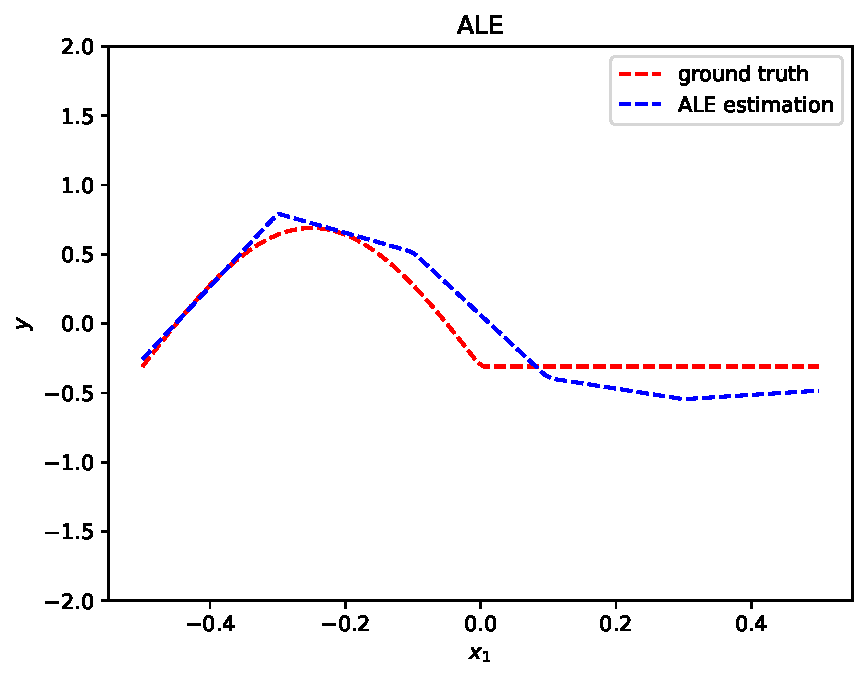
\includegraphics[width=0.49\textwidth]{./../code/concept_figure/exp_1_ale_5_bins_0.pdf}
          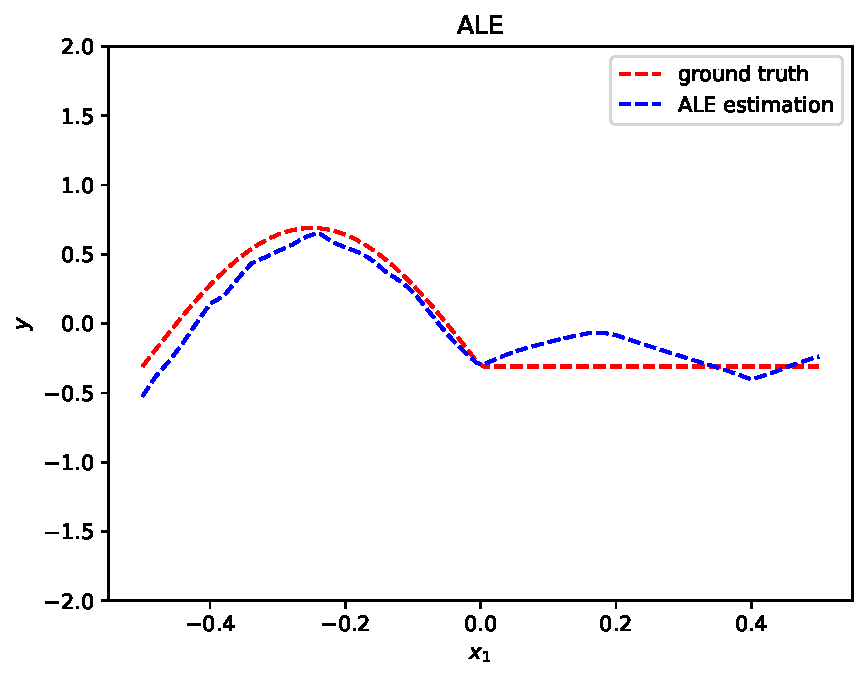
\includegraphics[width=0.49\textwidth]{./../code/concept_figure/exp_1_ale_50_bins_0.pdf}
          \caption{Left: ALE approximation with a narrow bin-splitting (5 bins). Right: ALE approximation with a dense bin-splitting (50 bins)}
          \label{fig:acc-1}
        \end{figure}
        \begin{itemize}
        \item Both approximations are bad:
          \begin{itemize}
          \item Narrow bin-splitting hides fine-grain details
            \item Dense bin-splitting is noisy (low samples per bin rate)
          \end{itemize}
          \item No information regarding the heterogeneity
        \end{itemize}
			\end{block}


      %%%%%% DALE vs ALE
      \begin{defbox}{Simple approach: ALE + Heterogeneity}{}

        \begin{tcolorbox}[ams equation*, title=ALE main effect definition]
            f^{\mathtt{ALE}}(x_s) = \int_{x_{s,\min}}^{x_s} \underbrace{\mathbb{E}_{X_c|X_s=z}\left [f^s (z, X_c)\right ]}_{\mu(z)} \partial z
        \end{tcolorbox}

        \begin{tcolorbox}[ams equation*, title=ALE main effect approximation]
          \hat{f}^{\mathtt{ALE}}(x_s) =
          \Delta x \sum_k^{k_x} \underbrace{\frac{1}{|\mathcal{S}_k|}
            \sum_{i:\xb^i \in \mathcal{S}_k} [\frac{\partial
                f}{\partial x_s}(x_s^i, \bm{x^i_c})]}_{\text{bin effect}: \hat{\mu}(z)}
        \end{tcolorbox}

        \begin{tcolorbox}[ams equation*, title=ALE heterogeneity definition]
          \sigma(x_s) = \sqrt{\int_{x_{s,\min}}^{x_s} \underbrace{\mathbb{E}_{X_c|X_s=z}\left [ \left (f^s (z, X_c) - \mu(z) \right )^2 \right ] \partial z}_{\sigma^2(z)}}
        \end{tcolorbox}


        \begin{tcolorbox}[ams equation*, title=ALE heterogeneity approximation]
  \mathtt{STD}(x_s) = \sqrt{\sum_{k=1}^{k_x} (z_k - z_{k-1})^2 \underbrace{\frac{1}{|\mathcal{S}_k| - 1}
\sum_{i:\mathbf{x}^i \in \mathcal{S}_k} \left ( f^s(\mathbf{x}^i) -
  \hat{\mu}(z_1, z_2) \right )^2}_{\hat{\sigma^2(z)}}}
        \end{tcolorbox}

  \end{defbox}

      %%%%%% DALE vs ALE
      \begin{defbox}{Simple but wrong: ALE + Heterogeneity}{}

        \begin{figure}
          \centering
          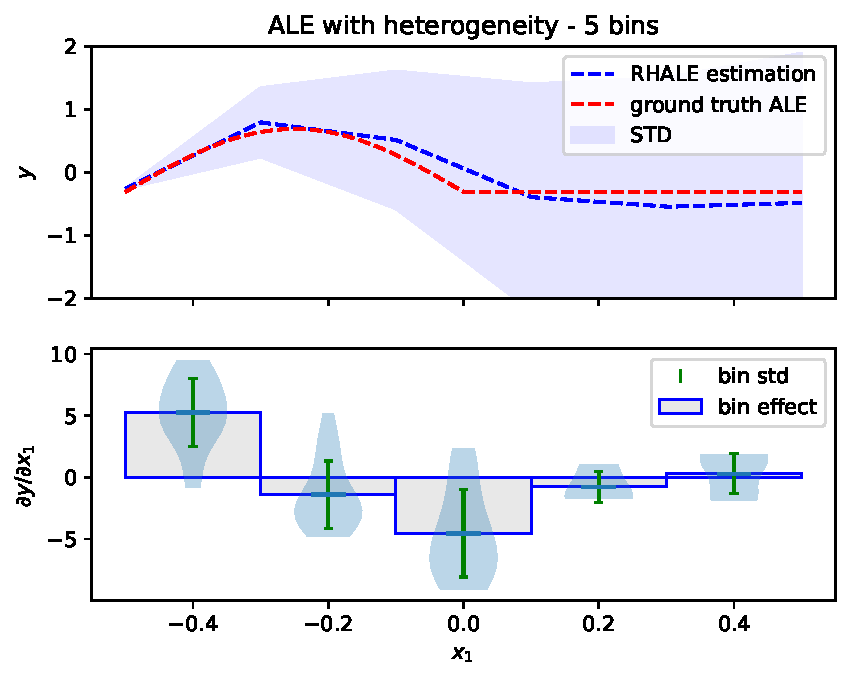
\includegraphics[width=0.49\textwidth]{./../code/concept_figure/exp_1_rhale_5_bins_0.pdf}
          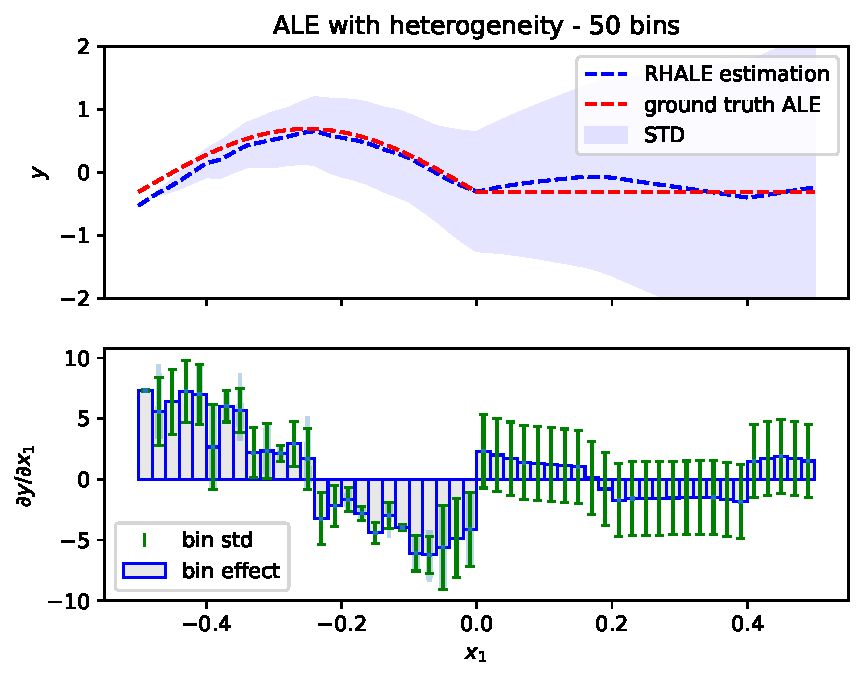
\includegraphics[width=0.49\textwidth]{./../code/concept_figure/exp_1_rhale_50_bins_0.pdf}
          \caption{Left: approximation with narrow bin-splitting (5 bins) and (Right) with dense-bin splitting}
          \label{fig:acc-1}
        \end{figure}

        \vspace{2mm}

        \begin{enumerate}
        \item Fixed-size bin splitting can ruin the estimation of the heterogeneity
        \end{enumerate}

  \end{defbox}

\end{column}

\separatorcolumn
\begin{column}{\colwidth}

  % DALE ACCURACY
  \begin{block}{RHALE: Robust and Heterogeneity-aware ALE}

    \begin{figure}
      \centering
      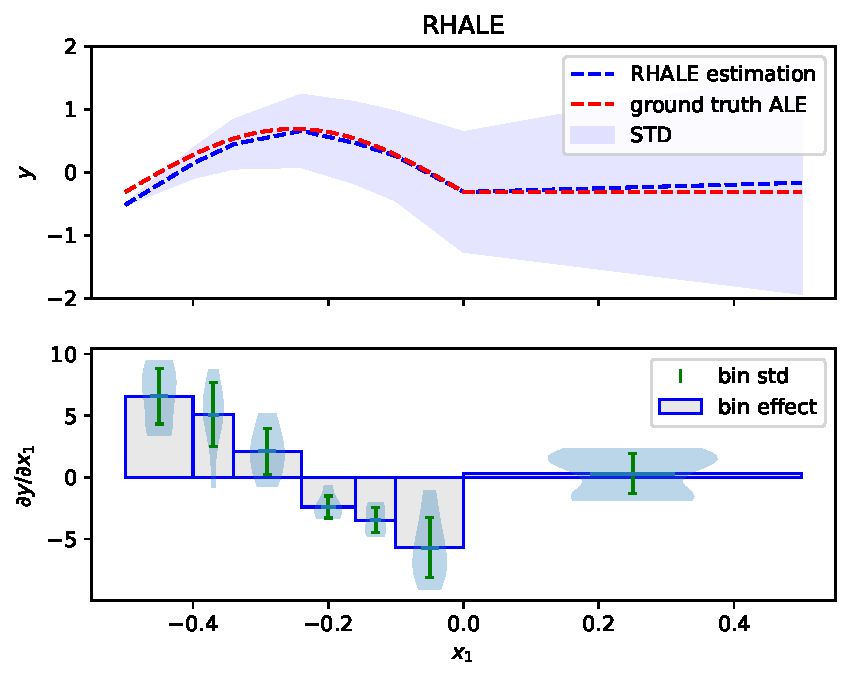
\includegraphics[width=0.95\textwidth]{./../code/concept_figure/exp_1_rhale_0.pdf}
      \caption{Narrow bins (\(K=40\)) \(\Rightarrow\) limited
        \(\frac{\text{samples}}{\text{bin}}\) \(\Rightarrow\) both plots are noisy }
      \label{fig:acc-1}
    \end{figure}

    \vspace{2mm}
    Simple but correct:
    \begin{itemize}
    \item Automatically finds the \textbf{optimal} bin-splitting
    \item Optimal $\Rightarrow$ best approximation of the average (ALE) effect
    \item Optimal $\Rightarrow$ best approximation of the heterogeneity 
    \end{itemize}
  \end{block}

      \begin{defbox}{Optimal bin-splitting}{}

        In the paper, we \textbf{formally prove}:  
        \begin{enumerate}
        \item the conditions under which a bin does not hide the finer details of the main effect
        \item the conditions under which a bin is an unbiased approximator of the heterogeneity

        \item that given (1) and (2), increasing bin size leads to a reduction in estimation variance
        \end{enumerate}

        \vspace{10mm}

        Based on the above, we formulate bin-splitting as an optimization problem and propose an efficient solution using dynamic programming.

  \end{defbox}

  
      \begin{alertblock}{Conclusion} In case you work with a differentiable model, as in Deep Learning, use RHALE to:
        \begin{itemize}
        \item quantify the heterogeneity of the ALE plot, i.e., the deviation of the instance-level effects from the average effect
        \item get a robust approximation of (a) the main ALE effect and (b) the heterogeneity, using automatic bin-splitting
      \end{itemize}
    \end{alertblock}

    \begin{block}{References}
      \begin{itemize}
      \item \large Paper repo: \href{git@github.com:givasile/RHALE.git}{git@github.com:givasile/RHALE.git}
      \item \large Personal site: \href{givasile.github.io}{givasile.github.io}
      \item \large Twitter: \href{https://twitter.com/givasile1}{twitter.com/givasile1}
      \end{itemize}
    \end{block}

    \begin{figure}
      \centering
      
\includegraphics[width=0.49\textwidth]{./Publications.png}
    \end{figure}

\end{column} \separatorcolumn
\end{columns}

% \begin{columns}[t]\separatorcolumn
%     \begin{column}{1.3\colwidth}
%       \large
% 	\end{column} \separatorcolumn
% 	\begin{column}{0.7\colwidth}
% \end{column}
% \separatorcolumn
% \end{columns}


\end{frame}

\end{document}